\label{chp:results}

After introducing the implementation of the \emph{ab initio} Green Kubo (aiGK) method in the previous chapter, we are now in position to present results for the set of potential thermal insulators identified in chapter~\ref{chp:anharmonicity}.

We first discuss the question of simulation time convergence for an initial set of materials in order to predict systems which can be computed with a simulation time of 30-60\,ps. This time was chosen as a compromise between the finite amount of available computational ressources, and the desire to compute as many materials from the list of candidates as possible.
% 57 materials
%
In a second step, we compare the computed thermal conductivities at room temperature to experimental references for the subset of materials where experiments are available to further verify the aiGK method beyond the two materials presented in the previous chapter.
% 22 materials 
%
In the last step, we present the computed thermal conductivities for the remaining materials,~i.\,e.,~those where no experimental thermal conductivity was reported before, and discuss how they fit into the schema of predicting thermal insulators from anharmonicity estimation as discussed in Sec.\,\ref{sec:kappa_vs_sigmaA}.
\idea{we highlight some materials with noteworthy properties and try to answer some open question in the experimental literature}

\idea{compare to theoretical approaches, i.e., the Roekeghem perovskites}



\section{Convergence estimation}
We discuss simulation time convergence in the light of the \emph{effective simulation time} introduced in Sec.\,\ref{sec:implementation.convergece}. The key idea is to identify lower boundaries for the \emph{necessary} effective simulation time in a material in order to asses whether a time-converged thermal conductivity is possible to obtain within a simulation time of 30-60\,ps. The rational for this approach is that for individual materials, one would always compute several times longer trajectories to ensure that all relevant contributions are captured. In turn, several times less materials could be computed with a given amount of computational resources. Here, we leverage observations across different materials to circumvent this necessity for individual materials, thereby allowing to compute good estimates for thermal conductivity for dozens of them.

We choose materials based on the criteria displayed in Fig.\,\ref{fig:results.convergence} based on converged thermal conductivities in 7 materials. We define four thresholds of minimal effective simulation time based on a material's anharmonicity $\sigmaA$, reflecting that phonons in harmonic materials like MgO have longer lifetimes than those in anharmonic materials.
%
\begin{figure}
	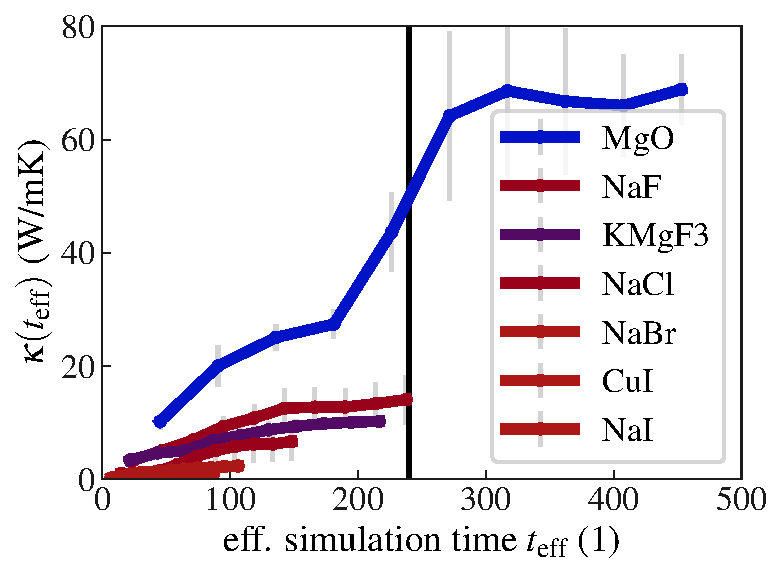
\includegraphics[width=.49\textwidth]{./data/plots/kappa_convergence/3.pdf}
	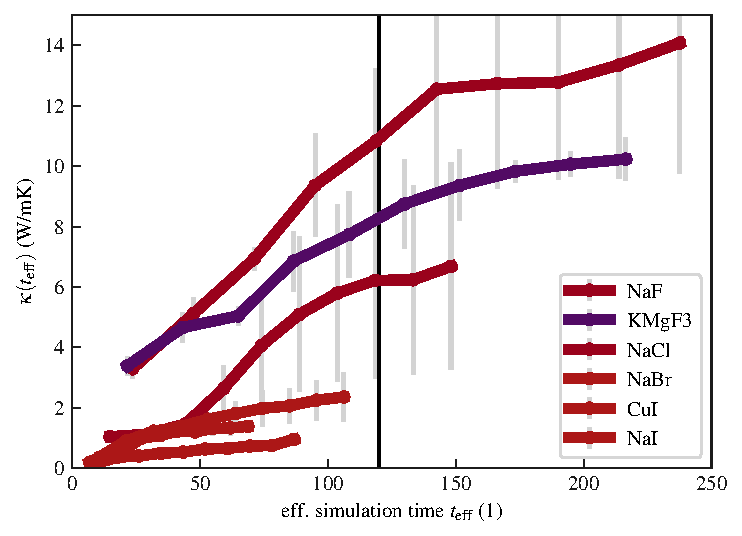
\includegraphics[width=.49\textwidth]{./data/plots/kappa_convergence/4.pdf}
	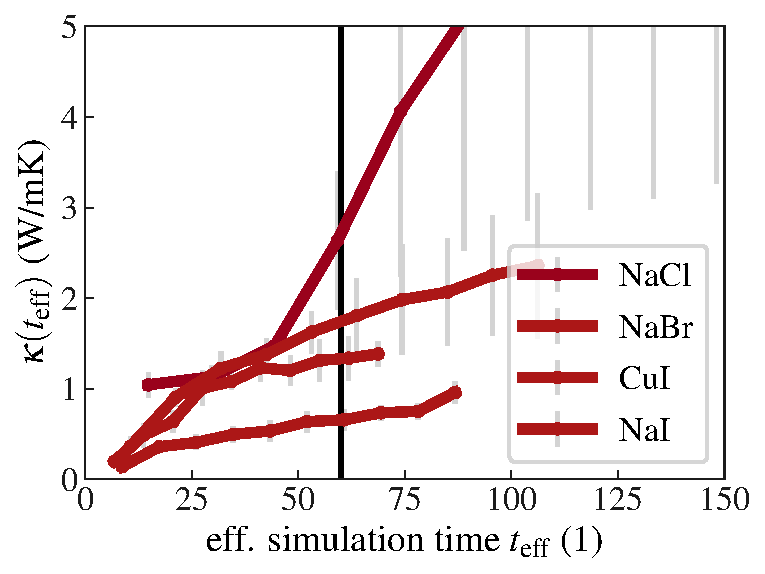
\includegraphics[width=.49\textwidth]{./data/plots/kappa_convergence/5.pdf}
	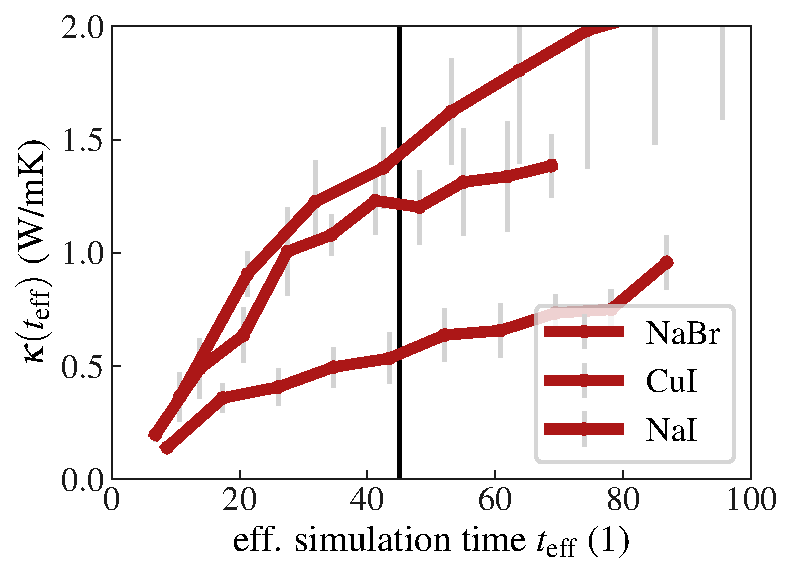
\includegraphics[width=.49\textwidth]{./data/plots/kappa_convergence/6.pdf}
	\caption{Illustration of minimal necessary effective simulation times. Upper left: $\teff = 240$ for harmonic materials with $\sigmaA \leq 0.2$. Upper right: $\teff = 120$ for materials with $0.2 < \sigmaA \leq 0.3$. Lower left: $\teff = 60$ for materials with $0.3 < \sigmaA \leq 0.4$. Lower right: $\teff = 45$ for materials with $\sigmaA > 0.4$.}
	\label{fig:results.convergence}
\end{figure}
%
We point out that at this stage, the given thresholds are meant as a \emph{necessary} condition for convergence, which ensures that a significant contribution to the cumulative thermal conductivity is included in the simulation. A statement about the \emph{sufficient} simulation time, however, can only made on the level of individual trajectories and should therefore be reserved for the verification of materials that show interesting properties after the \emph{necessary} simulation time.

Based on this estimation, we identify \todo{fill}XX~materials out of the list of \todo{fill}XXX~candidates to compute thermal conductivity on, and discuss those in the following.
\REM{list of materials in appendix}



\section{Comparison to Experiment}
In order to further asses the validity of the aiGK method for the computation of thermal conductivity in anharmonic compounds, we compare results for 21 materials to the experimental literature. A detailed list including all considered experimental references is given in Tab.\,\ref{tab:kappa.exp} in appendix~\ref{sec:app.experiments}. The difficulties when comparing to experimental references haven been discussed in detail for periclase MgO in Sec.\,\ref{sec:mgo.experiments}. In principle, these carry over to all other compounds, however, for most materials, the body of literature is much smaller compared to MgO. The list of experiments also includes measurements on polycrystalline samples. While thermal conductivity should be reduced in polycrystalline samples compared to single crystals because of boundary scattering, experimental studies have shown that the effect is minor in sufficiently dense polycrystalline samples, especially in low thermal conductivity materials~\cite{charvat1957}. In the course of our literature review we have generally found differences of 0-20\,\% between measurements on single- and polycrystalline samples, which supports this finding. Nevertheless, additional care must be taken when evaluating literature on polycrystalline samples: Some experiments specifically aim at reproducing polycrystalline samples of near-bulk density in order to assess the bulk thermal conductivity of a material. Experiments aiming at measuring other properties, in particular the thermoelectric figure of merit, typically do not attempt to reproduce the bulk thermal conductivity, and use less dense samples. The resulting thermal conductivity will then be influenced severely by the details of the sample processing, and a comparison to bulk thermal conductivity is not meaningful. The experiments on polycrystalline samples considered in this work are of the former type.

A comparison of thermal conductivities computed via the aiGK method as introduced in the previous chapter and the experimental literature is shown in Fig.\,\ref{fig:kappa_exp}.
%
\begin{figure}
	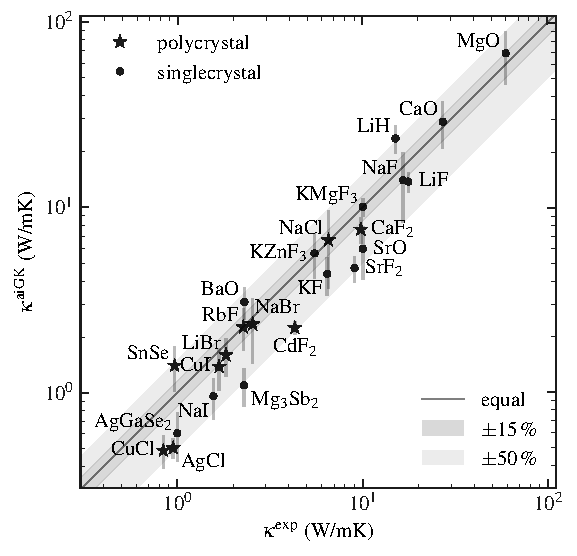
\includegraphics[width=\textwidth]{./data/plots/kappa_vs_exp_trusted/kappa_vs_exp_corrected_annotated.pdf}
	\caption{Comparison to experiment. Bullets($\bullet$): Single crystal. Stars ($\star$): Contains data from polycrystalline experiment. Error bar in y-direction: Statistical uncertainty for $\kappa^{\rm aiGK}$ from standard error over individual trajectories. Diagonal line: Agreement with experiment or mean of experiments if multiple available. Dark grey region: Agreement between mean experiment and mean computation with $\pm 15\,\%$ deviation. Light grey region: Agreement between mean experiment and mean computation with $\pm 50\,\%$ deviation.}
	\label{fig:kappa_exp}
\end{figure}
%
We find overall very good agreement in the 21 considered materials, with 10 out of 21 being within experimental accuracy of $\pm 15\,\%$, and all other within an ``extended experimental accuracy'' which we choose as $\pm 50\,\%$ within the average experimental reference, reflecting the high degree of variation in experimental values for materials where a significant amount of references is available, see especially the discussion in Ref.\,\cite{wei2016}. 

\begin{marginfigure}
	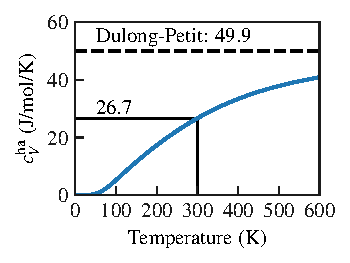
\includegraphics[width=\textwidth]{./data/plots/heat_capacity/225.LiH/thermal_properties.pdf}
	\caption{Harmonic heat capacity per formula unit $c_V^{\rm ha}$ for LiH compared to the classical Dulong-Petit value.}
	\label{fig:LiH.cv}
\end{marginfigure}
%
The strongest deviation from experiment is seen for LiH, which is computed as $\kappa^{\rm aiGK} = 23.6 \pm 4.0$\,W/mK, where the available experimental value is $\kappa^{\rm exp} = 14.7$\,W/mK~\cite{slack1973}. However, both lithium and especially hydrogen are light elements, so that LiH is not fully classical at room temperature, as can be estimated by comparing the harmonic heat capacity of LiH at 300\,K to the classical Dulong-Petit value in Fig.\,\ref{fig:LiH.cv}~\cite{Dove}. The harmonic heat capacity for LiH is only at about 50\,\% of the classically expected value of $6 R = 49.9$\,J/mol/K for solids with two atoms in the unitcell. This value can only be taken as an upper boundary to the deviation in thermal tranpsort properties expeceted from the lack of nuclear quantum effects (NQE), since low-frequency phonon modes already behave more classical at the given temperature.  A significant overestimation by the classical Green Kubo method can nevertheless be expected in this material. Interestingly, the aiGK value agrees very well with another computational study by Lindsay, who found a value of $\kappa = 23.00$\,W/mK using third-order Boltzmann transport~\cite{lindsay2016}. In that approach, the quantum nature of nuclei should be better captured than in the aiGK method, so that Lindsay ascribes the deviation from experiment to higher-order phonon-phonon interactions neglected in their approach, which is in line with the more phenomenological discussion proposed by Slack in Ref.\,\cite{slack1973}, who points out the strong anharmonicity in LiH that manifests in the change of phonon frequencies as measured by the Gr\"uneisen parameter. Indeed, in this study we find a value of $\sigmaA = 0.30$ for the strength of anharmonicity in LiH, which can be expected to be even larger when nuclear quantum effects are considered.\footnote{NQE increase the anharmonic strength of LiH at room temperature to about $\sigmaA = 0.36$~\cite{hengst1}.} We therefore suggest LiH as an interesting yet simple candidate for studying the interplay of strong anharmoncity and nuclear quantum effects in bulk solids in future work.


\section{New materials and relation to anharmonicity}
After validating the aiGK method against experimental literature, we present results for \todo{fill}XX~materials \emph{without} experimental reference. We display these values in the context of the $\kappa$ vs. $\sigmaA$ plot introduced in Fig.\,\ref{fig:anh.kappa}, where we identified a power-law relation of experimental thermal conductivities with the anharmonicity measure $\sigmaA$ for simple elementary and binary materials. We show the data again in Fig.\,\ref{fig:kappa_sigma_exp_comp}, but this time including the additional, non-experimentally measured materials computed in this work.
%
\begin{marginfigure}
	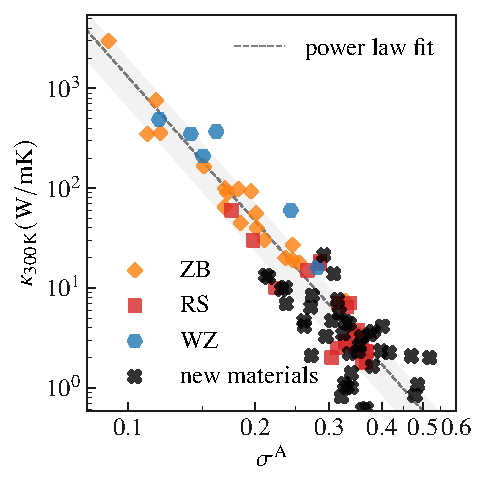
\includegraphics[width=\textwidth]{./data/plots/anharmonicity/9_kappa/incl_computations/sigma_vs_kappa_annot_comp_margin.pdf}
	\caption{Thermal conductivity at room temperature vs. anharmonicity measure.}
	\label{fig:kappa_sigma_exp_comp}
\end{marginfigure}
%
It is apparent that the correlation between thermal conductivity $\kappa$ and $\sigmaA$ carries over from the simple materials to the more complex binary and ternary compound classes studied in this work, since the power-law fit in Fig.\,\ref{fig:kappa_sigma_exp_comp} is still performed with respect to the experimental values presented in Fig.\,\ref{fig:anh.kappa}.


Focusing on the new materials, we show a zoomed-in part of the $\kappa-\sigmaA$ plane in Fig.\,\ref{fig:kappa_sigma}, with only computational data, highlighting the materials where no experimental reference is available.
%
\begin{figure}
	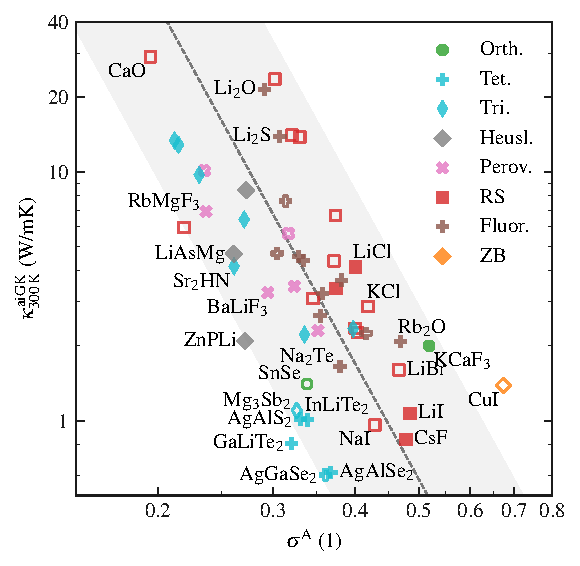
\includegraphics[width=\textwidth]{./data/plots/kappa_vs_sigma_trusted/kappa_vs_sigma_trusted_experiment.pdf}
	\caption{Thermal conductivity at room temperature computed via \emph{ab initio} Green Kubo (aiGK) vs. anharmonicity measure. Filled symbols denote materials without experimental reference. Open symbols represent materials where experimental reference is available.}
	\label{fig:kappa_sigma}
\end{figure}
%
In particular, we find 28 new materials with a computed bulk thermal conductivity of $\kappa^{\rm aiGK} < 10\,{\rm W/mK}$, 24 of which show $\kappa^{\rm aiGK} < 5\,{\rm W/mK}$, and 8 with $\kappa^{\rm aiGK} \leq 2\,{\rm W/mK}$. A full list of all values is given in Tab.\,\ref{tab:kappa.noexp}. The materials of very low thermal conductivity comprise simple binary, cubic materials such as the rock salt structures CsF ($\kappa^{\rm aiGK} = 0.84$) and LiI ($\kappa^{\rm aiGK} = 1.07$), or the fluorite structure Na$_2$Te ($\kappa^{\rm aiGK} = 1.64$). 

Particularly noteworthy is a class of ternary materials, so-called \emph{chalcopyrites}, a tetragonal crystal class closely related to the zincblende structure~\cite{wasim1979}. These crystals have been studied in the past primarily because of their non-linear optical properties~\cite{ho2014}, but also thermal transport properties have been studied~\cite{spitzer1970,wasim1979,garbato1979}, mainly because thermal transport can limit the optical efficiency in these devices~\cite{beasley1994}. However, experimental references for this class of materials are scarce, and do not agree well~\cite{beasley1994}. 
%
\begin{table}[ht]
  \centering
  \fontfamily{ppl}\selectfont
  \begin{tabular}{lc}
    \toprule
    Reference & Thermal conductivity \\
    & at 300\,K (W/mK) \\
    \midrule
    Berger 1966~\cite{berger1969}   & $2.7$ \\
    Beasley 1995~\cite{beasley1994} & $1.1$ \\
    This work                       & \prelim{$0.5 \pm 0.2$}  \\
    \bottomrule
    \vspace{.5em}
  \end{tabular}
  \caption{Overview of experimental references for AgGaSe$_2$. \inlinecomment{update values}.}
  \label{tab:exp.aggase2}
\end{table}
%
Picking AgGaSe$_2$ as an example, there are two distinct measurements available as summarized in Tab.\,\ref{tab:exp.aggase2}, ranging from $1.1-2.7$\,W/mK~\cite{beasley1994,berger1969}. These values are complemented by calculated values based on semi-empirical models, ranging from $4.8-9.0$\,W/mK~\cite{wasim1979,rincon1995}. Our computed thermal conductivities are collected in Tab.\,\ref{tab:exp.chalcopyrites}.
%
\begin{table}[ht]
  \centering
  \fontfamily{ppl}\selectfont
  \begin{tabular}{lrr}
    \toprule
    Material & $\kappa^{\rm aiGK}$ & $\sigmaA$ \\
    \midrule
        AgAlS$_2$   & \prelim{$0.84 \pm 0.13$} & 0.33 \\
        AgAlSe$_2$  & \prelim{$0.49 \pm 0.13$} & 0.37 \\
        AgGaSe$_2$  & \prelim{$0.53 \pm 0.13$} & 0.35 \\
        LiGaTe$_2$  & \prelim{$0.74 \pm 0.05$} & 0.31 \\
        LiInTe$_2$  & \prelim{$0.85 \pm 0.10$} & 0.33 \\
    \bottomrule
    \vspace{.5em}
  \end{tabular}
  \caption{Overview of computed thermal conductivities for chalcopyrite materials.}
  \label{tab:exp.chalcopyrites}
\end{table}
%
Besides AgGaSe$_2$, there is experimental reference the closely related material, AgGaS$_2$, with a measured thermal conductivity of 1.4\,W/mK~\cite{beasley1994}.\footnote{While we included AgGaS$_2$ in our dataset, we needed to discard the material because of aiMD convergence problems. However, we like to mention this material in the context of this study as potentially interesting material for future investigations.} While our computational data might underestimate the thermal conductivity in these compounds slightly\footnote{Please keep in mind, that the absolute errors are only of the order of 0.5-1\,W/mK.}, we nevertheless see a clear indiciation of very low intrinsic thermal conductivity in AgGaSe$_2$, and the chemically closely related compounds AgAlS$_2$ and AgAlSe$_2$. At least regarding their thermal transport properties, they are therefore comparable to the thermoelectric material Mg$_3$Sb$_2$~\cite{kajikawa2003,condron2006,zhang2009,zhang2018,pan2020,ding2021}.
\todo{$\kappa_{\rm MgSb}^{\rm aiGK} = 1.10 \pm 0.26$}

To elucidate the nuclear dynamics of the chalcopyrite systems, we present phonon spectral functions obtained from a temperature dependent model Hamiltonian for the nuclear system up to third-order displacements to estimate phonon-phonon interactions in Fig.\,\ref{fig:sqe_all}~\cite{Hellman2013,Hellman2013b,Squires}.
%
\begin{figure}
	\centering
	AgGaSe2$_2$ \hspace{3.7cm} AgAlSe$_2$\\
	% \includegraphics[width=0.49\textwidth]{./data/plots/spectral_functions/122.04.AgGaS2.12.png}
	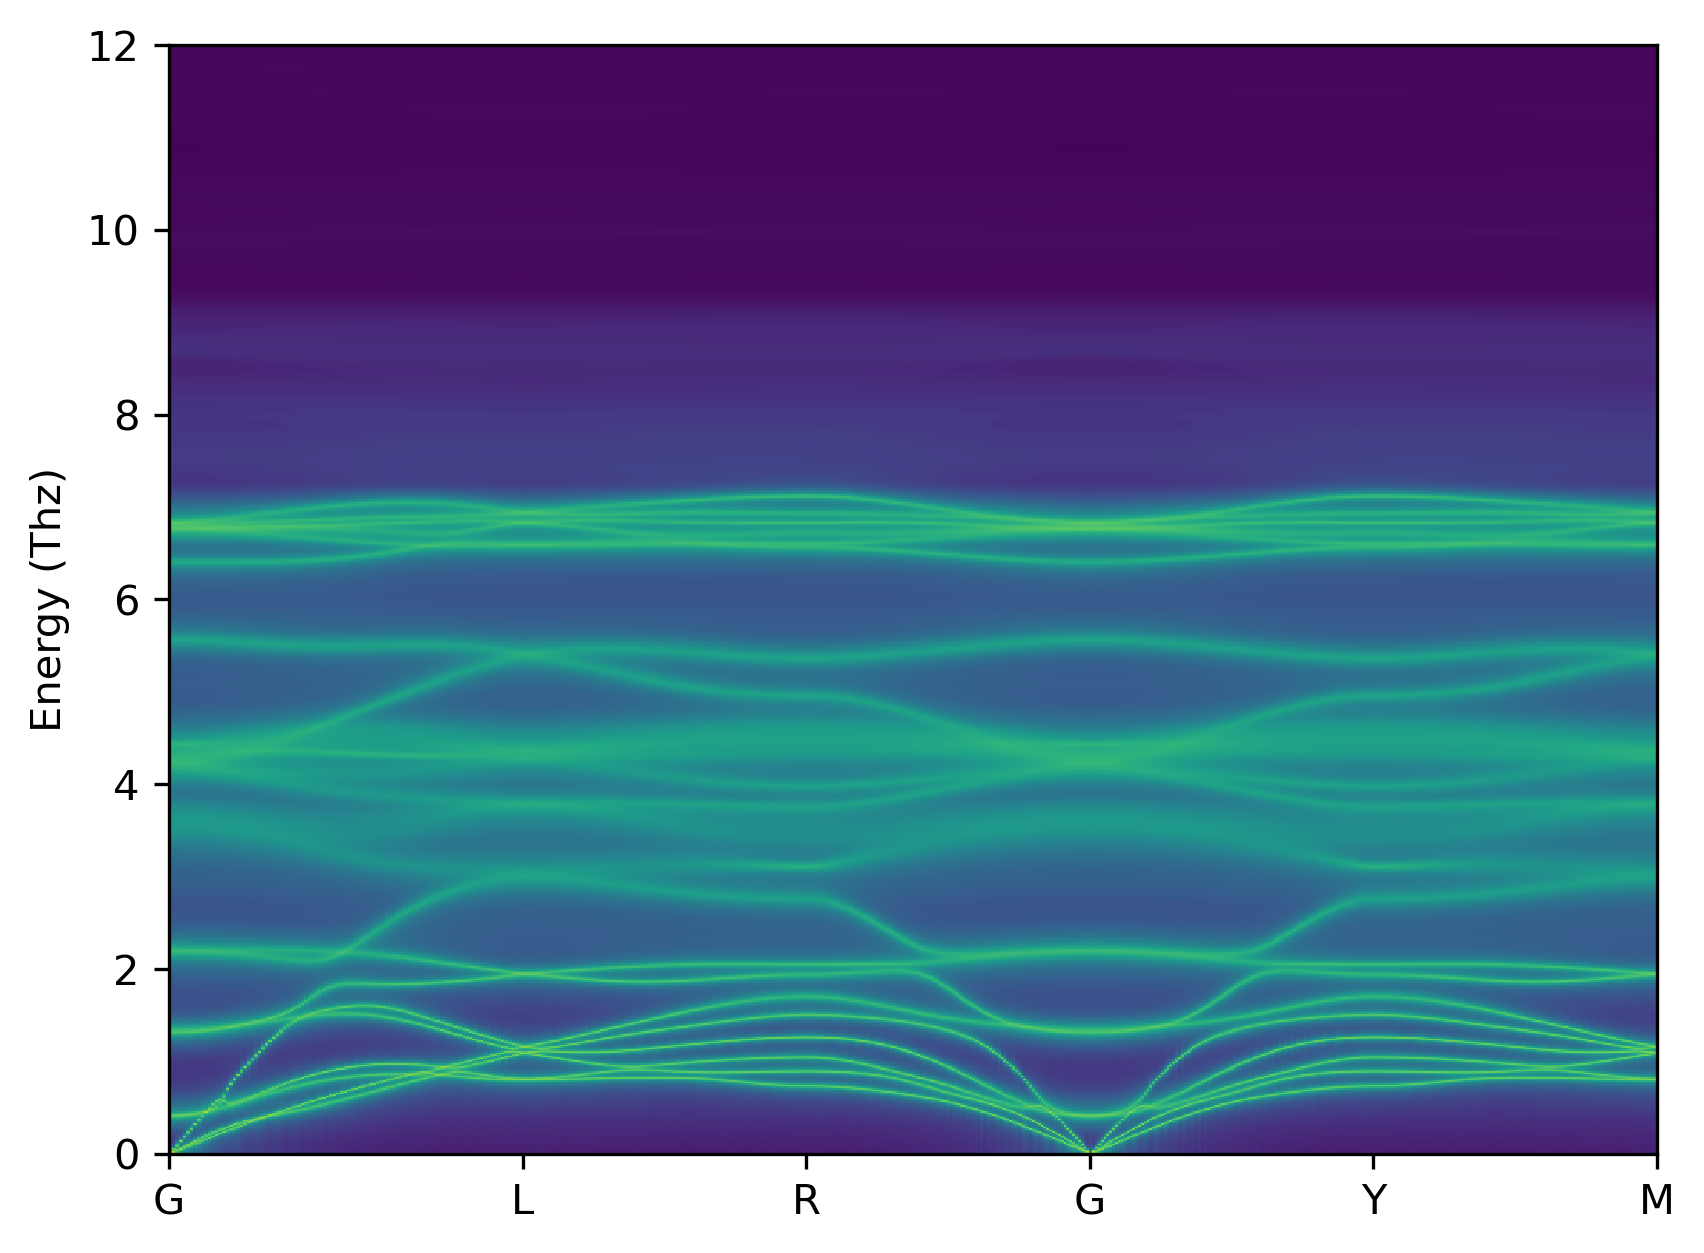
\includegraphics[width=0.49\textwidth]{./data/plots/spectral_functions/122.04.AgGaSe2.12.png}
	%	AgAlS$_2$ \hspace{3.7cm} AgAlSe$_2$\\
	%\includegraphics[width=0.49\textwidth]{./data/plots/spectral_functions/122.04.AgAlS2.15.png}
	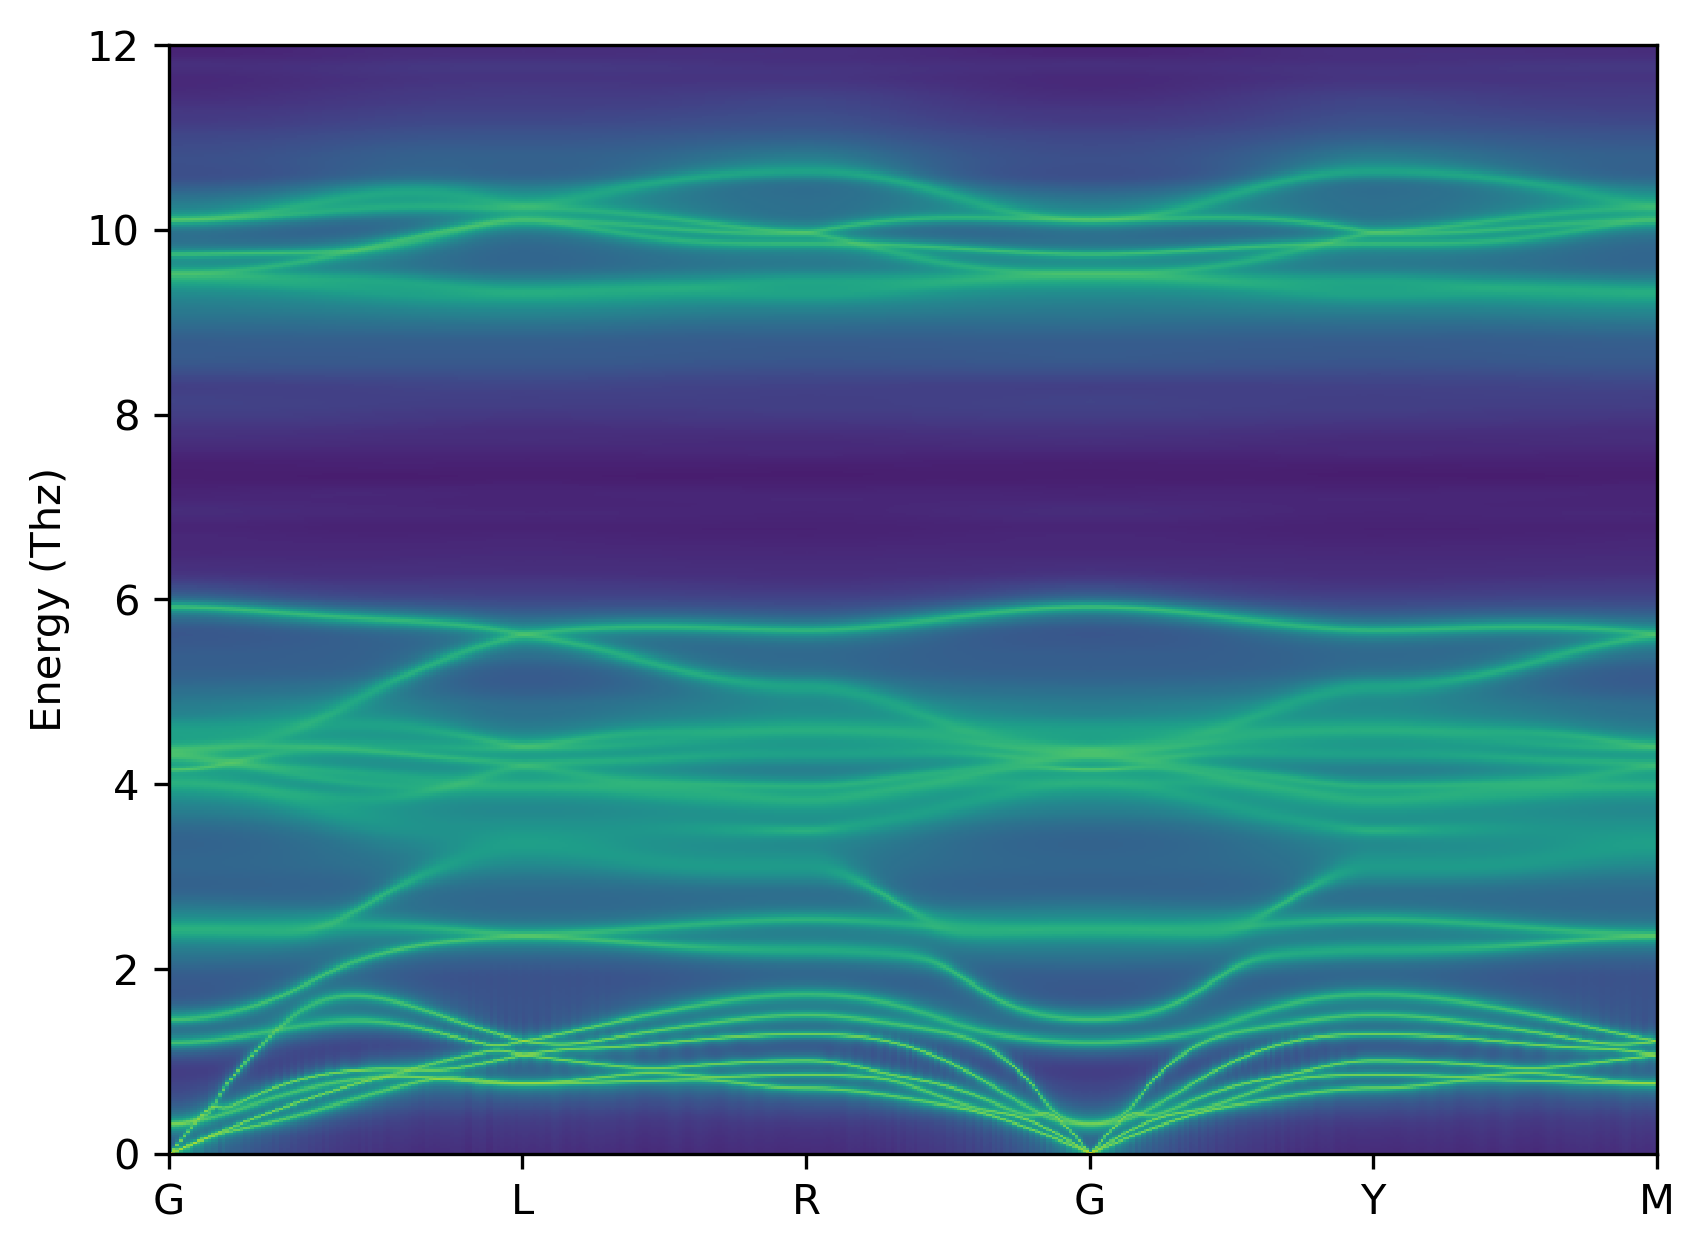
\includegraphics[width=0.49\textwidth]{./data/plots/spectral_functions/122.04.AgAlSe2.12.png}
	\\
	GaLiTe$_2$ \hspace{3.7cm} InLiTe$_2$\\
	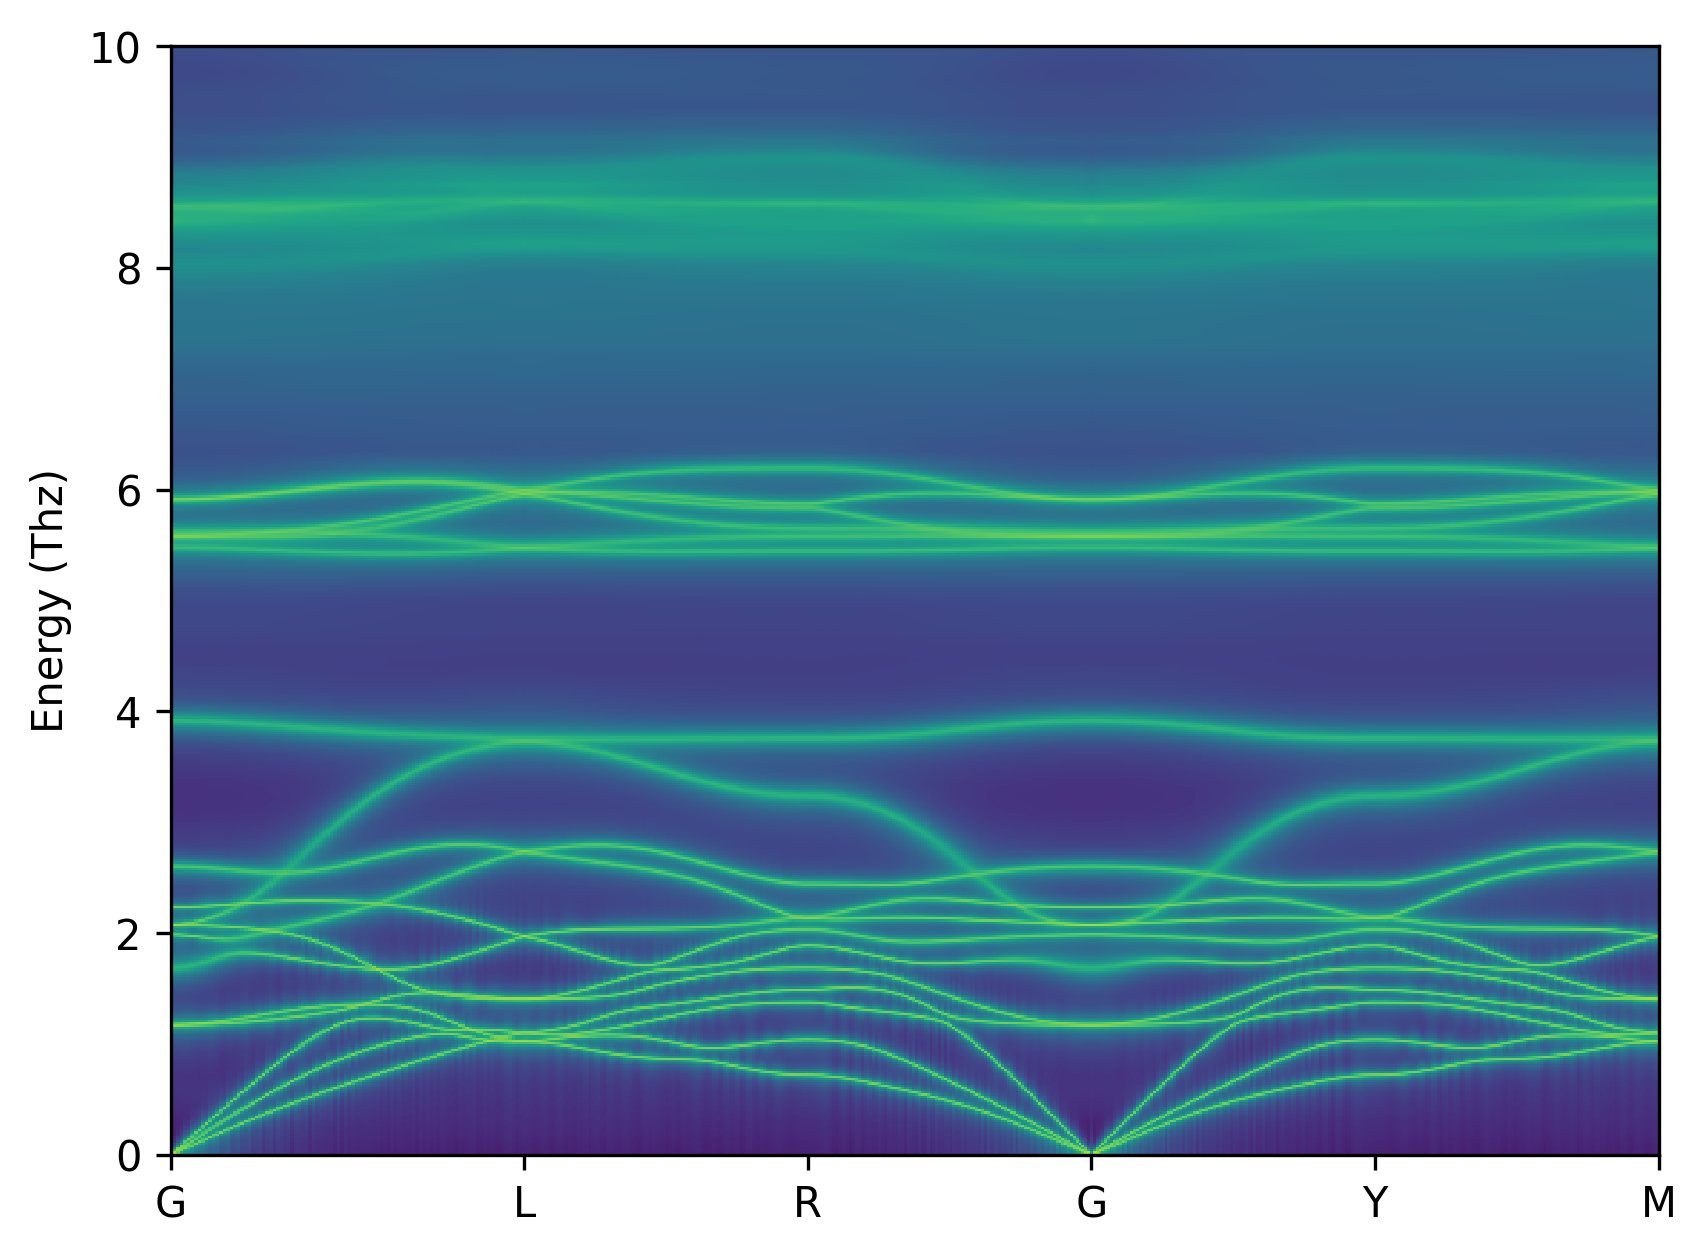
\includegraphics[width=0.49\textwidth]{./data/plots/spectral_functions/122.04.GaLiTe2.png}
	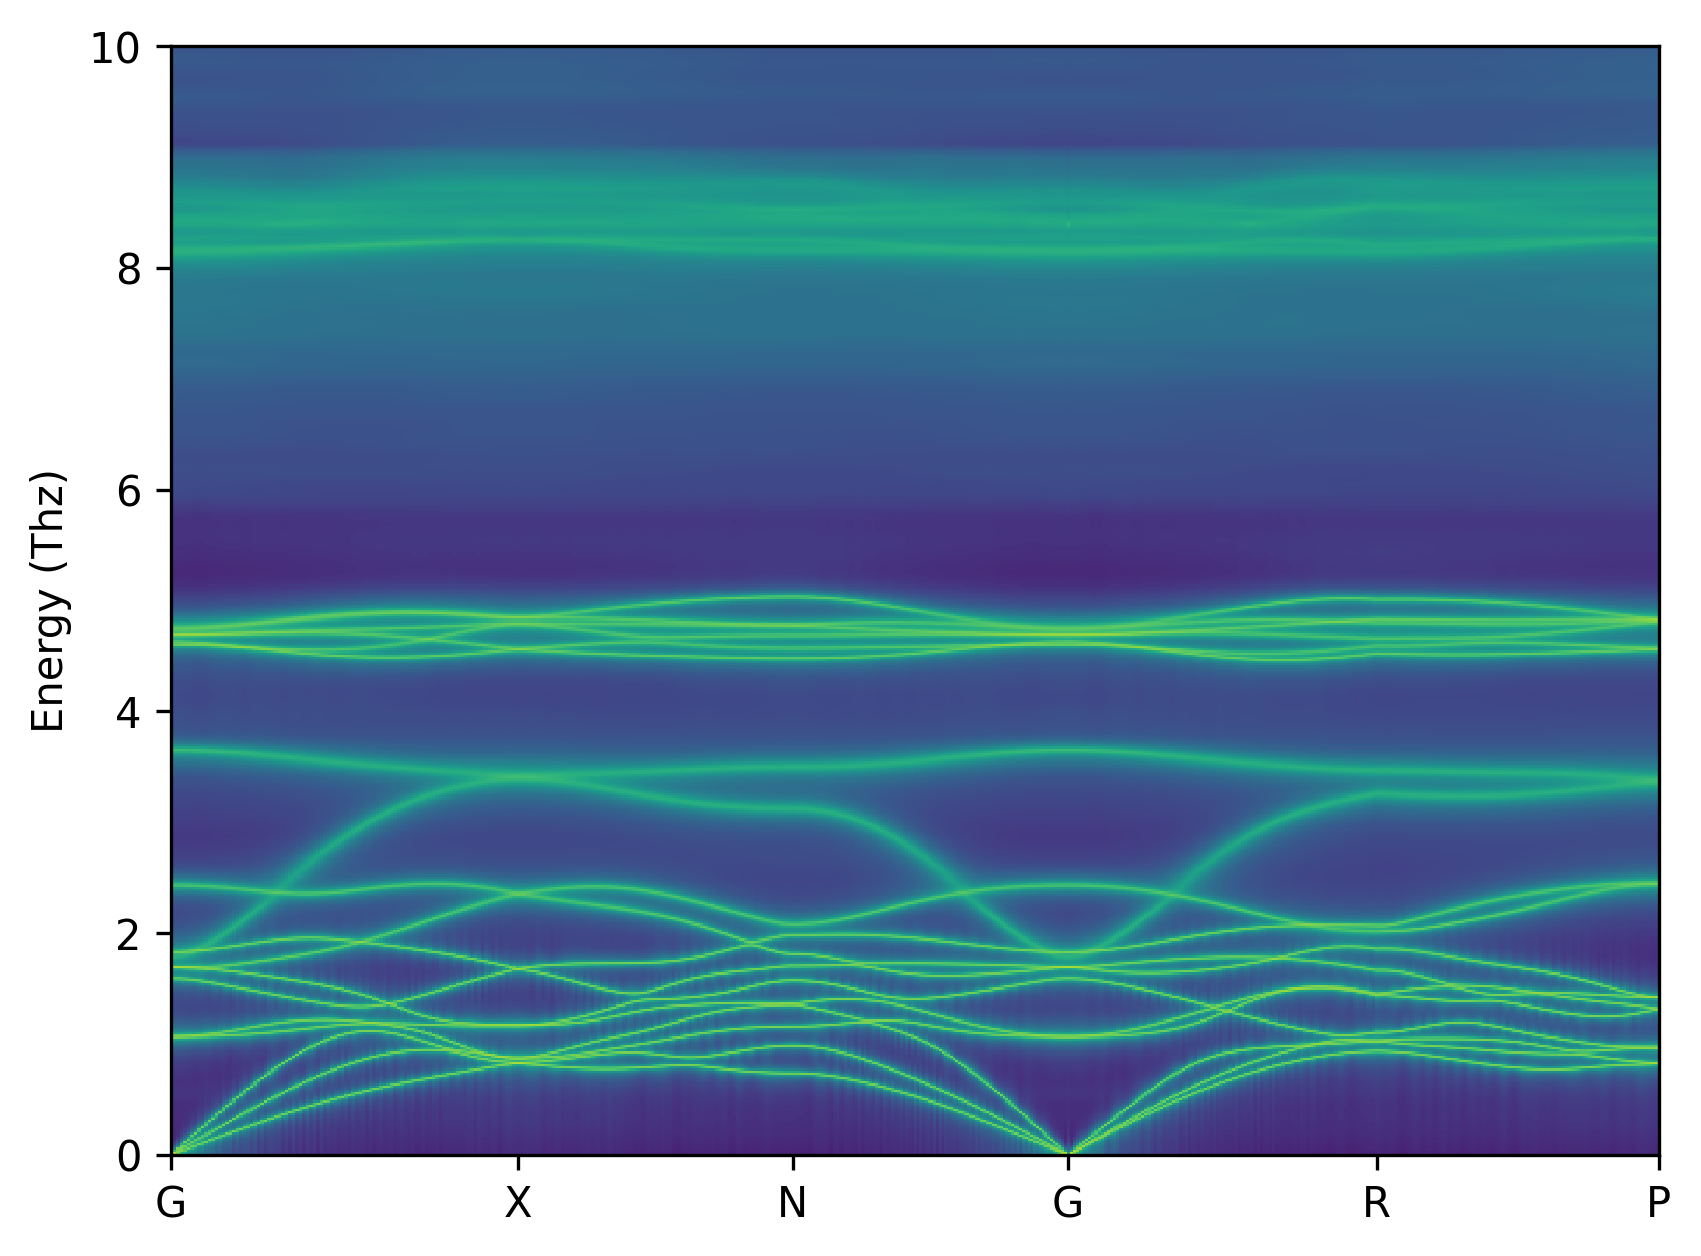
\includegraphics[width=0.49\textwidth]{./data/plots/spectral_functions/122.04.InLiTe2.png}
	\caption{Spectral functions for the chalcopyrite materials, AgGaSe$_2$, AgAlSe$_2$, GaLiTe$_2$, and InLiTe$_2$.}
	\label{fig:sqe_all}
\end{figure}
%
The common feature of these dispersions are the very flat acoustic branches which vary less than 1\,THz across the entire Brillouin zone, and a multitude of flat, nearly degenerate optical branches showing very litte to no dispersion. From a phonon-theory point of view, non-dispersive branches correspond to localized atomic motion in the system and therefore carry little heat beyond the Einstein-like diffusion of thermal energy from atom to atom, which is the dominant heat transport mechanism in structurally disordered systems like glasses~\cite{Simoncelli2019}. Furthermore, in particular the optical branches are substantially broadened, which corresponds to strong anharmonic coupling in these systems, reducing their thermal conductivity.

\begin{table}[ht]
  \centering
  \fontfamily{ppl}\selectfont
\begin{tabular}{rrrr}
\toprule
Space group  &    material & $\kappa^{\rm aiGK}$ & $\sigmaA$  \\
\midrule
         122 &  InLiTe$_2$ &                0.46 &       0.33 \\
         122 &  GaLiTe$_2$ &                0.47 &       0.31 \\
         122 &   AgAlS$_2$ &                0.84 &       0.33 \\
         122 &   FILL CHALCOPYRITES &       ---- &       ---- \\
         225 &         CsF &                0.84 &       0.48 \\
         225 &         LiI &                1.07 &       0.49 \\
         225 &    Na$_2$Te &                1.64 &       0.38 \\
          62 &    KCdF$_3$ &                1.67 &       0.53* \\
          62 &    KCaF$_3$ &                2.00 &       0.52 \\
         225 &     Rb$_2$O &                2.08 &       0.47 \\
         216 &       ZnPLi &                2.09 &       0.27 \\
         166 &  InNaSe$_2$ &                2.22 &       0.34 \\
         221 &   CsCdF$_3$ &                2.30 &       0.35 \\
         166 &  InLiSe$_2$ &                2.34 &       0.40 \\
         225 &    Na$_2$Se &                2.63 &       0.35 \\
         225 &    Li$_2$Te &                3.24 &       0.36 \\
         221 &   BaLiF$_3$ &                3.27 &       0.29 \\
         225 &          KH &                3.39 &       0.37 \\
         221 &   RbZnF$_3$ &                3.47 &       0.32 \\
         225 &      K$_2$O &                3.67 &       0.38 \\
         225 &        LiCl &                4.14 &       0.40 \\
         166 &    Sr$_2$HN &                4.17 &       0.26 \\
         225 &     Na$_2$S &                4.40 &       0.33 \\
         225 &    Li$_2$Se &                4.55 &       0.33 \\
         216 &      LiAsMg &                4.67 &       0.26 \\
         166 &   LiScS$_2$ &                6.42 &       0.27 \\
         221 &   RbMgF$_3$ &                6.94 &       0.24 \\
         216 &       LiNZn &                8.42 &       0.27 \\
         166 &   InNaO$_2$ &                9.71 &       0.23 \\
         166 &   CuGaO$_2$ &               12.82 &       0.22 \\
         166 &   LiRhO$_2$ &               13.37 &       0.21 \\
         225 &     Li$_2$S &               13.85 &       0.31 \\
         225 &     Li$_2$O &               21.39 &       0.29 \\
\bottomrule
\end{tabular}
  \caption{Bulk thermal conductivities for materials without experimental reference. *: The anharmonicity measure for KCaF$_3$ is increased when the entire simulation is taken into account with $\sigmaA \approx 1.32$, since the simulation is close to a structural phase transition. We observe jumps in $\sigmaA (t)$ similar to those discussed for KCaF$_3$ in Sec.\,\ref{chp:anharmonicity}, but more pronounced. When KCdF$_3$ is close to the orthorombic reference, $\sigmaA \approx 0.53$. Structural phase transition are known to occur in KCdF$_3$ at around 470\,K~\cite{hidaka1977,hidaka1990}.}
  \label{tab:kappa.noexp}
\end{table}
